%==============================================================================
%  Extrait pour relecture encadrante
%  Introduction générale + Chapitres 1 et 2 + Bibliographie
%  Compiler depuis le dossier rapport/ :
%    pdflatex extrait_ch1_ch2
%    biber extrait_ch1_ch2
%    pdflatex extrait_ch1_ch2
%    pdflatex extrait_ch1_ch2
%==============================================================================
\documentclass[12pt,a4paper,oneside]{report}

\usepackage[utf8]{inputenc}
\usepackage[T1]{fontenc}
\usepackage{lmodern}
\usepackage[french]{babel}
\usepackage{csquotes}
\babelhyphenation{régulation}

\usepackage[a4paper,top=2.5cm,bottom=2.5cm,left=3cm,right=2.5cm]{geometry}
\usepackage{setspace}
\onehalfspacing
\usepackage{parskip}

\usepackage{graphicx}
\usepackage{booktabs}
\usepackage{array}
\usepackage{tabularx}
\usepackage{longtable}
\usepackage{multirow}
\usepackage{float}
\usepackage{xcolor}
\usepackage{colortbl}
\usepackage{enumitem}

\usepackage{amsmath}
\usepackage{amssymb}

\usepackage{tikz}
\usetikzlibrary{arrows.meta,positioning,shapes.geometric,calc,fit,backgrounds}

\usepackage{fancyhdr}
\setlength{\headheight}{15pt}
\pagestyle{fancy}
\fancyhf{}
\fancyhead[L]{\nouppercase{\leftmark}}
\fancyfoot[C]{\thepage}
\renewcommand{\headrulewidth}{0.4pt}
\renewcommand{\footrulewidth}{0pt}
\fancypagestyle{plain}{%
  \fancyhf{}%
  \fancyfoot[C]{\thepage}%
  \renewcommand{\headrulewidth}{0pt}%
  \renewcommand{\footrulewidth}{0pt}%
}
\makeatletter
\let\ps@chapter\ps@plain
\makeatother

\usepackage[Lenny]{fncychap}

\usepackage[french,nolistfiles,nohints]{minitoc}
\setcounter{minitocdepth}{2}

\newcommand{\titreduchapitre}[2]{%
  \chapter{\textbf{#1}}%
  \label{#2}%
  \minitoc
  \thispagestyle{plain}%
  \newpage
  \thispagestyle{fancy}}

\usepackage{hyperref}
\hypersetup{
  colorlinks=true,
  linkcolor=black,
  citecolor=blue!50!black,
  urlcolor=blue!50!black,
  pdftitle={EmoLearn — Extrait Introduction, Chapitres 1 et 2},
  pdfauthor={BRIKI Maram}
}

\usepackage[backend=biber,style=numeric-comp,sorting=nyt,maxbibnames=99]{biblatex}
\addbibresource{references.bib}

\newcommand{\emolearn}{\textsc{EmoLearn}}
\newcommand{\arediger}{\par\nobreak\vspace{2pt}%
  \emph{\small[Contenu à rédiger.]}\par\medskip}

\begin{document}
\dominitoc

\begin{center}
  {\Large\textbf{\emolearn{}}}\\[0.6em]
  {\large Extrait pour relecture}\\[0.3em]
  {\normalsize Introduction générale --- Chapitres 1 et 2}\\[0.2em]
  {\normalsize Table des figures --- Liste des tableaux --- Bibliographie}\\[0.5em]
  {\normalsize BRIKI Maram}\\[0.2em]
  {\small Version de travail}
\end{center}
\vspace{0.8em}
\noindent\textit{Note.} Cet extrait contient l'Introduction générale, le
chapitre~1 (Fondements), le chapitre~2 (État de l'art), la table des figures,
la liste des tableaux et la bibliographie citée. Les renvois vers les
chapitres ultérieurs peuvent apparaître non résolus.

\pagenumbering{roman}
\renewcommand{\contentsname}{\textbf{Table des matières}}
\tableofcontents

\clearpage
\phantomsection
\addcontentsline{toc}{chapter}{Table des figures}
\mtcaddchapter
\renewcommand{\listfigurename}{\textbf{Table des figures}}
\listoffigures

\clearpage
\phantomsection
\addcontentsline{toc}{chapter}{Liste des tableaux}
\mtcaddchapter
\renewcommand{\listtablename}{\textbf{Liste des tableaux}}
\listoftables

\clearpage
\pagenumbering{arabic}

% Introduction générale (non numérotée) + sync minitoc pour Ch.1 / Ch.2
%==============================================================================
%  INTRODUCTION GÉNÉRALE — non numérotée (avant le chapitre 1)
%==============================================================================
\chapter*{\textbf{Introduction générale}}
\addcontentsline{toc}{chapter}{Introduction générale}
\mtcaddchapter % aligne le compteur minitoc (pas de Sommaire sur l'intro)
\label{chap:introduction}
\markboth{Introduction générale}{Introduction générale}
\thispagestyle{plain}

L'évolution rapide des technologies numériques et le développement des
plateformes éducatives en ligne ont profondément transformé les pratiques
d'apprentissage, en particulier à travers la diffusion des cours en ligne
ouverts et massifs (MOOC, \emph{Massive Open Online Courses}). Ces dispositifs
permettent aujourd'hui de collecter, diffuser et personnaliser des contenus
pédagogiques à grande échelle, offrant à des millions d'apprenants un accès
élargi à la formation, indépendamment des contraintes géographiques
\cite{breslow2013studying,daniel2012making}. La crise sanitaire de 2020 a
encore accéléré cette dynamique, faisant de l'apprentissage en ligne une
composante désormais structurelle des systèmes éducatifs contemporains.

Toutefois, cette évolution s'accompagne d'un constat largement documenté :
les MOOC souffrent de taux d'abandon particulièrement élevés. Une part
importante des inscrits interrompt son parcours dès les premières semaines,
ce qui limite fortement l'efficacité pédagogique réelle de ces dispositifs
\cite{onah2014dropout,jordan2015massive}. Parmi les facteurs explicatifs,
la baisse de l'\textbf{engagement} de l'apprenant occupe une place centrale
\cite{kizilcec2013deconstructing,hew2016promoting}. Dans une salle de classe
traditionnelle, l'enseignant perçoit en permanence des signaux fins (regard,
posture, expression) et adapte spontanément son discours. Cette boucle de
régulation disparaît presque entièrement dans les environnements en ligne de
masse, où l'apprenant fait face à un contenu figé, identique pour tous et
insensible à son état du moment.

Dans ce contexte, plusieurs travaux en informatique affective et en
psychologie de l'apprentissage ont établi que les émotions ne sont pas
périphériques à la cognition, mais en constituent un rouage essentiel
\cite{picard1997affective,pekrun2006control}. Des états tels que l'ennui, la
confusion ou la frustration influencent directement la profondeur du traitement
de l'information, la persévérance et la mémorisation
\cite{dmello2012dynamics,baker2010better}. Une détection inefficace de ces
états, combinée à l'absence d'adaptation pédagogique, peut entraîner une
dégradation de l'expérience d'apprentissage et favoriser le décrochage. Cette
problématique est d'autant plus critique que les décisions pédagogiques doivent
idéalement intervenir en temps utile, avant que le désengagement ne s'installe.

Ainsi, ce mémoire s'inscrit dans cette problématique en proposant une approche
visant à réunir, au sein d'une même chaîne de traitement, la perception de
l'engagement émotionnel et la génération adaptative de contenu pédagogique.

Face à ces enjeux, la question centrale de ce travail est la suivante :

\begin{center}
\textit{Comment concevoir un dispositif capable d'inférer automatiquement
l'état d'engagement d'un apprenant à partir de signaux multimodaux, puis de
générer en réponse un contenu pédagogique adapté à cet état, tout en
garantissant la cohérence et la traçabilité de la décision pédagogique
sous-jacente~?}
\end{center}

Cette question se décompose en quatre sous-questions opérationnelles :

\begin{itemize}
  \item Comment estimer de manière fiable l'état d'engagement à partir de
  signaux multimodaux hétérogènes (expressions faciales issues de
  \textsc{DAiSEE}, signal vocal issu de \textsc{IEMOCAP}), et quel gain la
  fusion apporte-t-elle par rapport à une modalité unique~?

  \item Comment formaliser une correspondance pédagogiquement justifiable
  entre les états d'engagement détectés et les stratégies d'intervention,
  c'est-à-dire un modèle \emph{engagement\,$\rightarrow$\,adaptation}~?

  \item Dans quelle mesure un grand modèle de langue, guidé par des patrons
  de prompts structurés et ancré par un mécanisme de récupération augmentée
  (RAG), peut-il produire un contenu pédagogique pertinent et adapté à l'état
  d'engagement visé~?

  \item Selon quel protocole peut-on évaluer, de façon honnête et
  multi-niveaux, la qualité de la perception, la pertinence de la décision et
  la qualité du contenu généré~?
\end{itemize}

L'analyse de la littérature montre que, malgré les progrès importants réalisés
dans les domaines de la détection de l'engagement et de l'IA générative
appliquée à l'éducation, ces deux axes restent majoritairement traités de
manière indépendante. D'une part, les modèles de perception multimodale
permettent d'inférer l'état affectif d'un apprenant avec une fiabilité
croissante \cite{dmello2015review,whitehill2014faces,gupta2016daisee}.
D'autre part, les grands modèles de langue ouvrent la voie à une génération
de contenu pédagogique personnalisée à grande échelle
\cite{brown2020language,kasneci2023chatgpt}. Cependant, ces approches
demeurent souvent séquentielles ou fragmentées~: la détection n'est pas
systématiquement reliée à une décision pédagogique explicite, tandis que la
génération n'est pas toujours conditionnée par un état d'engagement mesuré,
ce qui limite la capacité des systèmes à restaurer une forme de régulation
pédagogique automatique.

Pour répondre à ces limitations, ce mémoire propose un framework hybride nommé
\emolearn{}, combinant trois briques complémentaires. La couche de
\textbf{perception} estime l'état d'engagement à partir de signaux visage et
voix, en s'appuyant sur les corpus \textsc{DAiSEE} et \textsc{IEMOCAP} et sur
des modèles \emph{fine-tunés} vers la taxonomie des quatre états
d'engagement~: un Vision Transformer (ViT) pour le visage et un modèle
wav2vec2 pour la voix, combinés par un moteur de fusion multimodale. La couche
de \textbf{décision} formalise un modèle
\emph{engagement\,$\rightarrow$\,adaptation} reliant chaque état à un type de
contenu et à un patron de génération. Enfin, la couche de \textbf{génération}
produit un contenu pédagogique adaptatif au moyen d'un grand modèle de langue,
guidé par une bibliothèque de vingt patrons structurés et ancré par un module
RAG sur une base documentaire pédagogique. Ainsi, \emolearn{} vise à passer
d'un contenu figé à une adaptation réellement conditionnée par l'état
d'engagement détecté.

En résumé, le module de perception anticipe l'état émotionnel de l'apprenant,
tandis que les modules de décision et de génération exploitent cette estimation
pour produire une intervention pédagogique ciblée, traçable et reproductible.

Les principales contributions de ce travail sont les suivantes :

\begin{enumerate}
  \item Proposition d'une architecture multimodale de bout en bout reliant
  perception, décision et génération au sein d'une même chaîne.

  \item Formalisation d'un modèle \emph{engagement\,$\rightarrow$\,adaptation}
  assorti d'une bibliothèque de vingt patrons de génération structurés.

  \item Développement d'un module RAG pédagogique ancrant la génération sur
  une base documentaire vectorisée.

  \item Fine-tuning supervisé des modèles de perception (ViT pour le visage et
  wav2vec2 pour la voix) vers les quatre états d'engagement \textsc{DAiSEE}.

  \item Évaluation honnête et instrumentée de la fusion multimodale, incluant
  l'analyse des compromis entre exactitude globale et sensibilité aux états
  critiques.

  \item Prototype logiciel complet et reproductible, accompagné d'un protocole
  d'évaluation multi-niveaux.
\end{enumerate}

%==============================================================================
\section*{Méthodologie générale}
\label{sec:methodologie}

La démarche adoptée relève de la \emph{recherche orientée conception}
(\emph{design science research}), paradigme particulièrement adapté à la
conception d'artefacts informatiques répondant à un problème identifié
\cite{hevner2004design}. Elle articule l'analyse d'un problème réel (le
décrochage lié à la baisse d'engagement dans les MOOC), la construction
d'un artefact (le framework \emolearn{}) et son évaluation au regard
d'objectifs explicites.

Concrètement, le travail s'organise autour d'une chaîne de traitement en trois
étages : un étage de \emph{perception} (FER, SER, fusion), un étage de
\emph{décision} (règles temporelles et moteur pédagogique) et un étage de
\emph{génération} (RAG et LLM).

Le projet s'appuie sur deux corpus publics de référence. \textsc{DAiSEE}
\cite{gupta2016daisee} constitue le socle engagement (taxonomie et scénarios),
tandis qu'\textsc{IEMOCAP} \cite{busso2008iemocap} apporte la modalité vocale
et, via un sous-corpus audiovisuel aligné, le support de validation de la
fusion. Le prototype repose sur une architecture client-serveur, des modèles
de perception fine-tunés (ViT et wav2vec2) vers les quatre états
\textsc{DAiSEE}, un LLM accessible par API et un module RAG (ChromaDB).

%==============================================================================
\section*{Structure du mémoire}
\label{sec:structure}

Le présent mémoire s'ouvre par la présente \textbf{introduction générale},
puis s'organise en six chapitres numérotés.

Le \textbf{chapitre~1} pose les fondements conceptuels de l'apprentissage
adaptatif et de l'engagement (MOOC, émotions, détection multimodale, IA
générative).

Le \textbf{chapitre~2} propose un état de l'art critique et positionne
\emolearn{} par rapport aux travaux existants.

Le \textbf{chapitre~3} est consacré à la modélisation et à la conception du
framework : architecture globale, modèle
\emph{engagement\,$\rightarrow$\,adaptation}, génération fondée sur des patrons
et un module RAG, ainsi que conception du prototype.

Le \textbf{chapitre~4} décrit l'implémentation technique de bout en bout.

Le \textbf{chapitre~5} expose la validation et les résultats selon un protocole
multi-niveaux.

Le \textbf{chapitre~6}, enfin, synthétise les contributions, expose les limites
et trace des perspectives.

Le mémoire se termine par la bibliographie.


%==============================================================================
%  CHAPITRE 1 — FONDEMENTS
%==============================================================================
\titreduchapitre{Fondements de l'apprentissage adaptatif et de l'engagement}{chap:fondements}

%==============================================================================
\section{Introduction}
\label{sec:fond-intro}

La conception d'un système d'apprentissage adaptatif fondé sur
l'engagement émotionnel mobilise un ensemble de notions issues de
domaines distincts : sciences de l'éducation, informatique affective,
apprentissage multimodal et intelligence artificielle générative. Ces
notions sont souvent présentées séparément ; les rassembler permet
d'établir un vocabulaire partagé et d'expliciter les hypothèses sur
lesquelles repose le pipeline \emolearn{}.

Ce chapitre examine les concepts fondamentaux nécessaires à la
compréhension de cette architecture. Il aborde successivement
l'apprentissage en ligne et les MOOC, la notion d'engagement de
l'apprenant, les apports de l'informatique affective, les principes de
la détection multimodale, puis les bases de l'intelligence artificielle
générative appliquée à l'éducation (LLM, guidage par prompts et RAG).

%==============================================================================
\section{Apprentissage en ligne et MOOC}
\label{sec:fond-mooc}

\subsection{Définition}

Les cours en ligne ouverts et massifs (MOOC, \emph{Massive Open Online
Courses}) désignent des dispositifs de formation accessibles à distance, le
plus souvent sans prérequis d'inscription stricts, et destinés à un public
potentiellement très large \cite{daniel2012making,breslow2013studying}. Ils
reposent typiquement sur des vidéos pédagogiques, des quiz, des forums et un
parcours de progression asynchrone.

\subsection{Implication pour l'adaptation}

Dans ce modèle, le contenu est principalement diffusé de manière uniforme.
Toute forme d'adaptation automatique suppose donc, en amont, de disposer
d'une mesure d'engagement plus fine que les simples proxies de présence
(connexion, clics), point développé dans la section suivante.

%==============================================================================
\section{Engagement de l'apprenant}
\label{sec:fond-engagement}

\subsection{Définition}

L'engagement désigne la mobilisation cognitive, comportementale et
émotionnelle de l'apprenant vis-à-vis de la tâche d'apprentissage
\cite{kizilcec2013deconstructing,hew2016promoting,fredricks2004school}. Il ne se réduit pas à la
simple présence en ligne (connexion, clics), mais renvoie à une implication
active dans le traitement de l'information.

\subsection{Dimensions de l'engagement}

On distingue classiquement :


\begin{figure}[H]
\centering
\begin{tikzpicture}[
  box/.style={rectangle, rounded corners=3pt, draw=#1, thick, fill=#1!12,
              minimum width=3.6cm, minimum height=1.55cm, align=center,
              font=\small},
  arr/.style={-{Stealth[length=2.4mm]}, thick, gray!70}
]
\node[box=teal!70!black] (cog) {\textbf{Cognitif}\\profondeur du traitement\\stratégies d'apprentissage};
\node[box=blue!70!black, right=0.55cm of cog] (beh) {\textbf{Comportemental}\\participation\\persévérance};
\node[box=orange!80!black, right=0.55cm of beh] (emo) {\textbf{Émotionnel}\\intérêt, ennui,\\frustration, etc.};
\node[draw=gray!55, dashed, rounded corners=4pt, fit=(cog)(beh)(emo),
      inner sep=8pt, label={[font=\small\bfseries]above:Engagement de l'apprenant}] {};
\node[below=0.35cm of emo, font=\footnotesize\itshape, text=orange!80!black, align=center]
  {Focus \emolearn{}};
\end{tikzpicture}
\caption{Les trois dimensions classiques de l'engagement. }
\label{fig:fond-dimensions-engagement}
\end{figure}

\emolearn{} se concentre principalement sur la dimension émotionnelle /
affective, tout en visant un effet sur la persévérance globale.

\subsection{Mesure de l'engagement}

Les indicateurs usuels en e-learning (durée de session, progression, scores)
fournissent des \emph{proxies} utiles mais incomplets. Les approches plus
récentes mobilisent des signaux multimodaux (visage, voix, posture) pour
estimer l'état affectif de manière plus directe
\cite{dmello2015review,sharma2020multimodal,goldberg2021attentive}.

%==============================================================================
\section{Informatique affective et émotions en apprentissage}
\label{sec:fond-affect}

\subsection{Rôle des émotions dans l'apprentissage}

Les travaux en psychologie de l'apprentissage montrent que les émotions
modulent l'attention, la mémorisation et la persévérance
\cite{pekrun2006control,dmello2012dynamics,baker2010better,loderer2020beyond,graesser2020emotions}. Elles ne sont
donc pas périphériques à la cognition, mais constitutives du processus
d'apprentissage.

\subsection{États pertinents pour l'adaptation pédagogique}

Dans le cadre de ce mémoire, quatre états issus du corpus \textsc{DAiSEE}
\cite{gupta2016daisee} structurent la taxonomie d'engagement :


\begin{figure}[H]
\centering
\begin{tikzpicture}[
  etat/.style={rectangle, rounded corners=3pt, draw=#1, very thick, fill=#1!14,
               minimum width=3.5cm, minimum height=1.7cm, align=center, font=\small},
  arr/.style={-{Stealth[length=2.4mm]}, thick, gray!65}
]
\node[etat=green!55!black] (eng) {\textbf{Engagement}\\implication positive\\maintenir / enrichir};
\node[etat=gray!70!black, right=0.7cm of eng] (bor) {\textbf{Ennui}\\sous-stimulation\\relancer};
\node[etat=blue!65!black, below=0.65cm of eng] (con) {\textbf{Confusion}\\incompréhension\\clarifier};
\node[etat=red!65!black, right=0.7cm of con] (fru) {\textbf{Frustration}\\blocage\\soutenir / simplifier};
\node[draw=black!40, rounded corners=5pt, fit=(eng)(bor)(con)(fru),
      inner sep=10pt,
      label={[font=\small\bfseries]above:Taxonomie \textsc{DAiSEE} (4 états)}] {};
\end{tikzpicture}
\caption{Taxonomie des quatre états d'engagement retenus (\textsc{DAiSEE}).}
\label{fig:fond-taxonomie-daisee}
\end{figure}

Chacun de ces états appelle une stratégie pédagogique distincte.

\subsection{Charge cognitive}

La théorie de la charge cognitive rappelle qu'un contenu trop dense ou mal
séquencé favorise la confusion et l'abandon
\cite{sweller1988cognitive,sweller2019cognitive}. La théorie de
l'apprentissage multimédia complète ce cadre : la conception des messages
(texte, image, rythme) conditionne la charge utile
\cite{mayer2021multimedia}. L'adaptation du niveau d'explication, du rythme
et du type d'exemple constitue dès lors un levier central des systèmes
d'apprentissage adaptatifs.

%==============================================================================
\section{Détection multimodale de l'engagement}
\label{sec:fond-detection}

\subsection{Modalités exploitées}

La détection automatique de l'engagement peut s'appuyer sur :
\begin{itemize}
  \item le \textbf{visage} (expressions faciales, regard)~;
  \item la \textbf{voix} (prosodie, intensité, variations émotionnelles)~;
  \item éventuellement la posture ou des signaux physiologiques.
\end{itemize}
\emolearn{} combine les deux premières modalités, à partir de clips
vidéo et audio annotés (hors temps réel), plutôt que de traces textuelles
de forums ou de capteurs physiologiques.

\begin{figure}[H]
\centering
\begin{tikzpicture}[
  box/.style={rectangle, rounded corners=3pt, draw=black!70, thick,
              minimum width=2.5cm, minimum height=1.05cm, align=center, font=\small},
  io/.style={rectangle, rounded corners=2pt, draw=black!50, dashed,
             minimum width=2.4cm, minimum height=0.9cm, align=center, font=\footnotesize},
  arr/.style={-{Stealth[length=2.5mm]}, very thick, black!65}
]
\node[io] (vid) at (0,3.6) {Vidéo\\visage};
\node[io] (aud) at (4.2,3.6) {Audio\\voix};
\node[box, fill=blue!10] (fer) at (0,2.2) {FER};
\node[box, fill=blue!10] (ser) at (4.2,2.2) {SER};
\node[box, fill=teal!15] (fus) at (2.1,0.85) {Fusion\\multimodale};
\node[box, fill=orange!12] (etat) at (2.1,-0.55) {État\\d'engagement};
\node[box, fill=yellow!18] (adap) at (2.1,-1.95) {Adaptation\\pédagogique};

\draw[arr] (vid) -- (fer);
\draw[arr] (aud) -- (ser);
\draw[arr] (fer) -- (fus);
\draw[arr] (ser) -- (fus);
\draw[arr] (fus) -- (etat);
\draw[arr] (etat) -- (adap);
\end{tikzpicture}
\caption{Boucle conceptuelle de détection multimodale.}
\label{fig:fond-boucle-multimodale}
\end{figure}

\subsection{Corpus de référence}

Deux corpus publics fondent la chaîne de perception :
\begin{itemize}
  \item \textsc{DAiSEE} \cite{gupta2016daisee} pour l'engagement facial annoté~;
  \item \textsc{IEMOCAP} \cite{busso2008iemocap} pour l'émotion vocale et, via
  un sous-corpus audiovisuel, la validation de la fusion alignée.
\end{itemize}

\subsection{Fusion multimodale}

La fusion vise à combiner des sources hétérogènes pour obtenir une décision
plus robuste qu'une modalité seule
\cite{liang2024foundations,gandhi2023multimodal}. Elle soulève toutefois des
questions de pondération, de désaccord inter-modalités et de déséquilibre des
classes, qui seront traités dans la conception et la validation du système.

%==============================================================================
\section{IA générative pour l'éducation}
\label{sec:fond-ia}

\subsection{Grands modèles de langue}

Les grands modèles de langue (LLM, \emph{Large Language Models}) sont des
réseaux de neurones entraînés à prédire le prochain token d'une séquence à
partir d'un très grand corpus textuel
\cite{brown2020language,vaswani2017attention,wolf2020transformers,openai2023gpt4,dubey2024llama3}. Architecturée autour du
\emph{Transformer} décodeur, cette famille de modèles suit un pipeline
strictement séquentiel (figure~\ref{fig:fond-llm-arch}) : le texte d'entrée
est d'abord \emph{tokenisé} (mots ou sous-mots convertis en identifiants
numériques), puis ces identifiants passent dans une couche d'\emph{embeddings}
combinée à un encodage de position, avant d'entrer dans une pile de blocs
d'\emph{attention} et de couches \emph{feed-forward}. Une tête de langage
produit enfin la distribution sur le vocabulaire. La génération est
\emph{auto-régressive} : chaque token prédit est réinjecté pour produire le
suivant.

\begin{figure}[H]
\centering
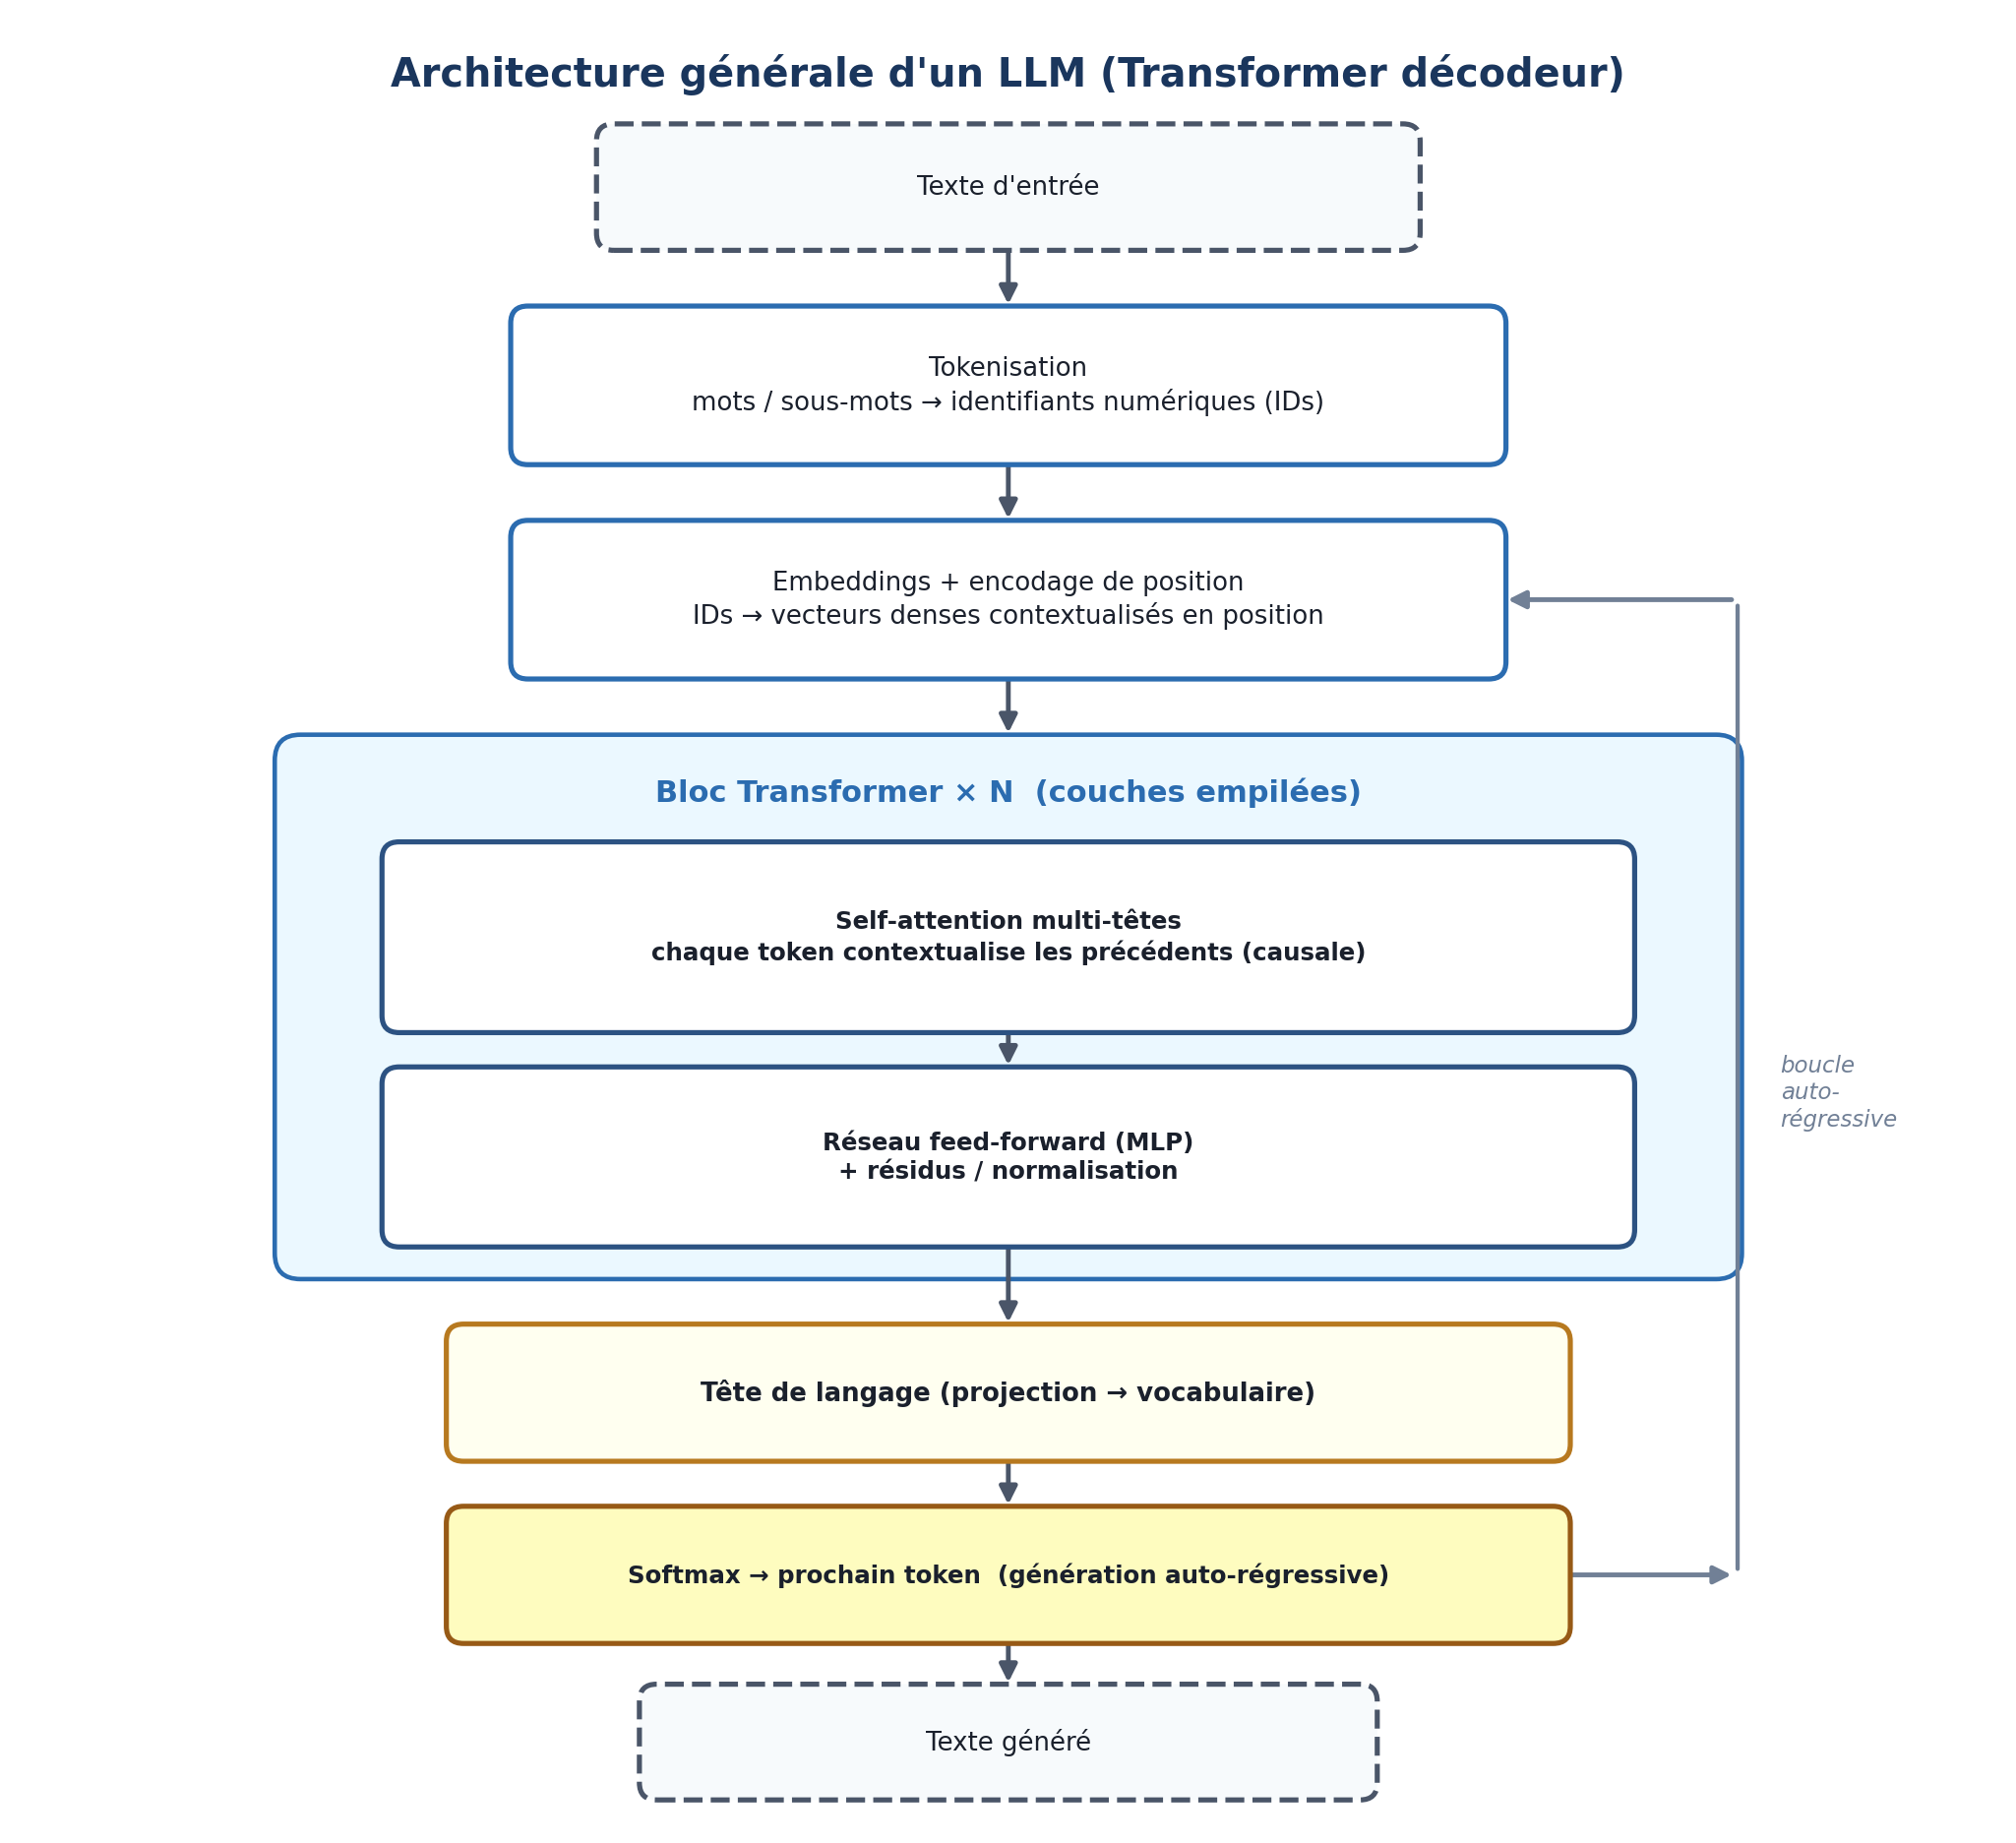
\includegraphics[width=0.88\textwidth]{figures/llm_architecture_generale.png}
\caption{Architecture générale d'un LLM de type Transformer décodeur.
}
\label{fig:fond-llm-arch}
\end{figure}

En éducation, ces modèles permettent de générer, à la demande, des
explications, reformulations, analogies ou encouragements en langage naturel
\cite{kasneci2023chatgpt,lo2023chatgpt,yan2024practical,wang2024large}. Ils offrent ainsi une voie crédible pour produire
des contenus pédagogiques personnalisés à grande échelle.

\subsection{Guidage par prompts et patrons}

La qualité du contenu généré dépend fortement du guidage
\cite{liu2023pretrain,white2023prompt,wei2022chain}. Une bibliothèque de
patrons de prompts structurés permet de conditionner la génération selon
l'état d'engagement détecté et le type d'intervention pédagogique souhaité.

\subsection{Récupération augmentée (RAG)}

Le mécanisme de \emph{Retrieval-Augmented Generation} (RAG)
\cite{lewis2020retrieval,gao2023retrieval,fan2024survey} ancre la génération sur des documents de référence
indexés dans une base vectorielle (figure~\ref{fig:fond-rag}). Les documents
sont d'abord découpés et vectorisés (indexation hors ligne). À l'exécution,
la question est embedée puis confrontée à l'index pour récupérer les
passages les plus pertinents ; ces passages enrichissent le prompt transmis
au LLM, qui produit une réponse ancrée. Ce dispositif réduit le risque
d'hallucinations factuelles et renforce la cohérence pédagogique des
contenus produits.

\begin{figure}[H]
\centering
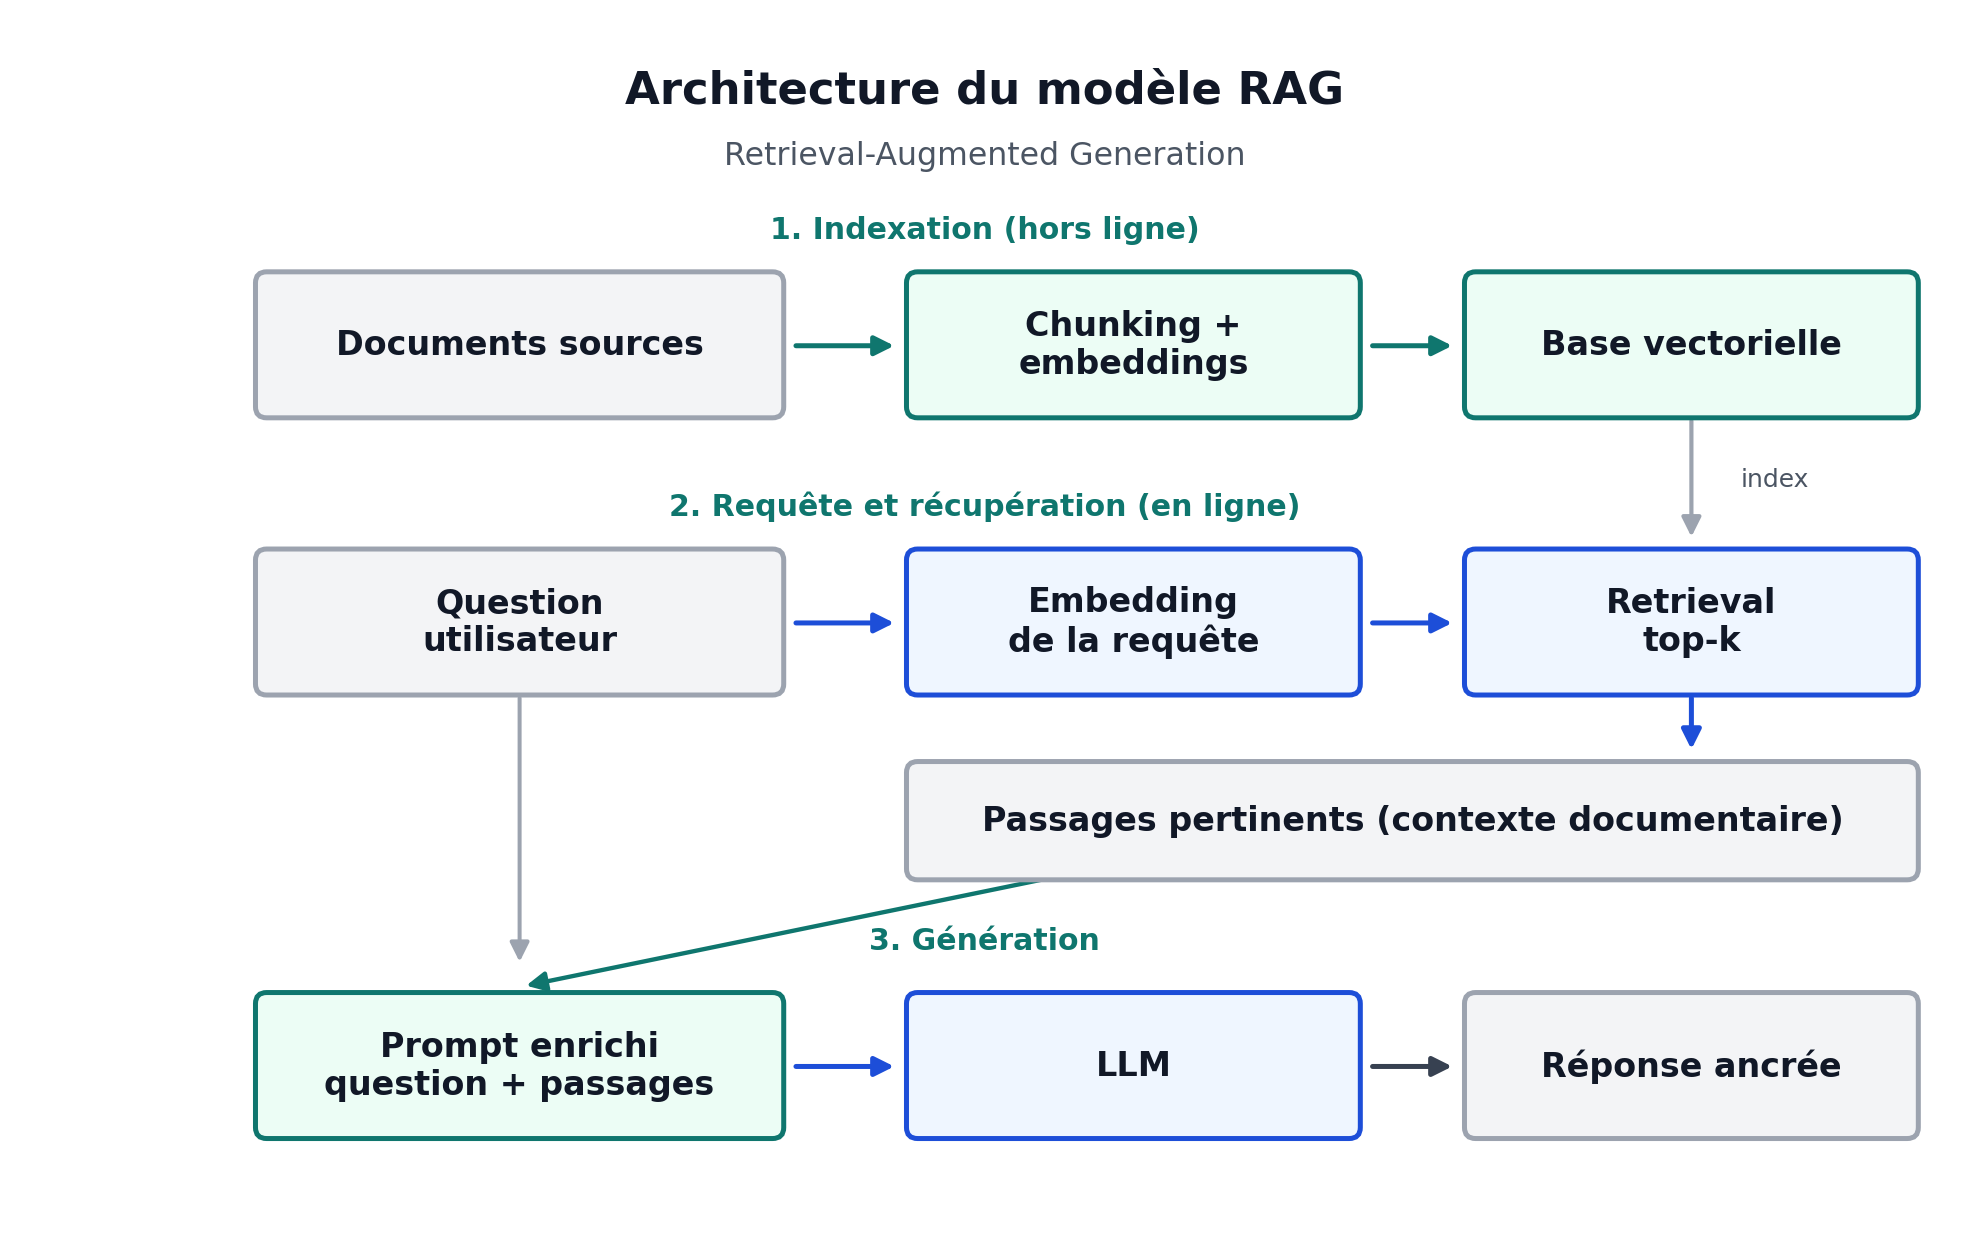
\includegraphics[width=0.92\textwidth]{figures/rag_architecture_generale.png}
\caption{Architecture générale du RAG.}
\label{fig:fond-rag}
\end{figure}

%==============================================================================
\section{Conclusion}
\label{sec:fond-concl}

Ce chapitre a rappelé le socle conceptuel sur lequel s'appuie \emolearn{} :
la définition des MOOC et l'enjeu d'adaptation, la centralité de
l'engagement émotionnel, les bases de la détection multimodale et le potentiel
de l'IA générative guidée et ancrée documentairement. Le chapitre suivant
examine l'état de l'art correspondant et positionne le présent travail par
rapport aux approches existantes.

%==============================================================================
%  CHAPITRE 2 — ÉTAT DE L'ART
%==============================================================================
\titreduchapitre{Synthèse de l'état de l'art}{chap:etat_art}

%==============================================================================
\section{Introduction}
\label{sec:ea-intro}

Le chapitre~\ref{chap:fondements} a fixé le vocabulaire. Il reste à
examiner ce que la littérature établit déjà, et ce qu'elle laisse ouvert,
lorsqu'il s'agit de réguler un apprenant isolé devant une vidéo de cours.

Deux familles de travaux se croisent sans se rejoindre pleinement. D'un
côté, on détecte l'engagement : parfois dans les messages de forum
(présence cognitive, émotions épistémiques), parfois sur le visage, la voix
ou la posture. De l'autre, on intervient : tuteurs intelligents,
règles d'adaptation, puis, depuis peu, texte généré par un grand modèle de
langue. Peu de prototypes enchaînent les deux : estimer un état, choisir une
stratégie, produire un contenu. C'est cet enchaînement que vise
\emolearn{}.

Le chapitre s'organise en six sections : MOOC et engagement apprenant,
détection automatique, psychologie des émotions, IA générative, systèmes
adaptatifs, puis synthèse critique et positionnement. Ce parcours prépare
les choix du chapitre~\ref{chap:conception}.

%==============================================================================
\section{MOOCs et engagement apprenant}
\label{sec:ea-mooc}

Trois questions structurent cette section : les défis de rétention, la
mesure de l'engagement en e-learning, puis les indicateurs émotionnels
et cognitifs.

\subsection{Défis de rétention et d'engagement}
\label{sec:ea-mooc-retention}

\textcite{daniel2012making} et \textcite{breslow2013studying}
ont d'abord décrit le MOOC comme un phénomène
d'accès ouvert à grande échelle. Les chiffres de rétention
sont connus depuis longtemps : une grande partie des inscrits part dans
les premières semaines, et le taux moyen d'achèvement stagne près de
10\,\% \cite{onah2014dropout,jordan2015massive,reich2019mooc}. Onah,
Jordan et Reich établissent ce constat. Kizilcec et Hew montrent que le
manque de temps n'explique pas à lui seul les départs : la baisse
d'engagement y contribue également
\cite{kizilcec2013deconstructing,hew2016promoting}. Le défi de rétention
porte donc aussi sur ce que les inscrits vivent pendant le cours, au-delà
du calendrier et du volume de travail déclaré.

\subsection{Mesure de l'engagement en e-learning}

L'engagement désigne la mobilisation cognitive, comportementale et
émotionnelle de l'apprenant sur une tâche \cite{fredricks2004school}. La
définition aujourd'hui la plus partagée distingue trois composantes :
\begin{itemize}
  \item l'engagement comportemental (participation, persévérance,
  effort observable)~,
  \item l'engagement cognitif (profondeur du traitement, stratégies
  d'apprentissage, présence cognitive)~,
  \item l'engagement émotionnel (intérêt, ennui, confusion,
  frustration, sentiment d'affiliation).
\end{itemize}
En e-learning, on mesure surtout des proxies : connexion, clics,
durée de session, progression, notes. Ils sont utiles, mais incomplets :
un étudiant peut rester connecté et être déjà ailleurs. Les journaux de
plateforme voient le comportement. Les forums donnent un aperçu de la
cognition, à condition que l'étudiant écrive. Compter les clics ne
suffit donc plus : il faut une mesure plus proche de ce que l'apprenant
est en train de vivre
\cite{kizilcec2013deconstructing,dmello2015review}.

\subsection{Indicateurs émotionnels et cognitifs}

L'émotion, pourtant liée à la persévérance
\cite{pekrun2006control,dmello2012dynamics}, n'apparaît pas dans les logs.
\emolearn{} s'appuie sur ces indicateurs, dans l'hypothèse qu'une
régulation plus précoce agit sur la suite du parcours. L'étude de Liu \emph{et al.} sur le forum d'\emph{Introduction
to Psychology} (8\,867 inscrits) va dans ce sens : émotion et cognition
bougent ensemble, et prédisent mieux la réussite lorsqu'on les lit
conjointement \cite{liu2022automated}. Un seul score d'\og engagement \fg{}
efface ces nuances.

Dès que l'on dispose de texte, la revue de Sakeef \emph{et al.} montre que
trois grilles reviennent pour coder l'engagement cognitif des
forums \cite{sakeef2025detecting}. La plus citée est le modèle de
Community of Inquiry \cite{garrison1999critical} : présence sociale,
enseignante et cognitive, cette dernière en quatre phases (déclenchement,
exploration, intégration, résolution). Hu \emph{et al.} et Liu \emph{et al.}
s'en servent pour entraîner des classifieurs
\cite{hu2021automatic,liu2023moocbert}. ICAP, proposé par Chi et Wylie,
classe plutôt le mode d'activité : passif, actif, constructif,
interactif \cite{chi2014icap}. Plus on construit ou on interagit, plus le
traitement est censé être profond.

Ces indicateurs cognitifs aident à relire un fil de discussion
après coup. Ils disent peu d'un visionnage sans contribution
écrite. Dans ce cas, les indicateurs émotionnels visibles, taxonomie
\textsc{DAiSEE} : engagement, ennui, confusion, frustration sont plus
directs : un état, un besoin pédagogique \cite{gupta2016daisee}.

%==============================================================================
\section{Détection automatique de l'engagement}
\label{sec:ea-detection}

On ne peut pas demander à un enseignant de coder des milliers de messages,
ni d'observer chaque visage. D'où l'intérêt d'un estimateur automatique.
Cette section examine trois axes : les approches multimodales (visuelle,
comportementale, physiologique), les corpus publics (\textsc{DAiSEE},
\textsc{EmotiW}, et les ressources complémentaires), puis les performances
rapportées dans la littérature. Les scores d'\emolearn{} lui-même (FER+AU,
WavLM, fusion) sont ceux du chapitre~\ref{chap:validation}, ils ne
constituent pas un palmarès de l'état de l'art.

\subsection{Approches multimodales}
\label{sec:ea-detection-multimodal}

D'Mello, dans sa méta-analyse, insiste sur un point pratique : ennui,
confusion, frustration et engagement reviennent souvent, et mélanger les
modalités aide, à condition de calibrer \cite{dmello2015review}. Trois
familles de signaux structurent cet axe.

\paragraph{Voie visuelle:}
En l'absence de production écrite, le signal disponible est celui que
l'on peut filmer. Whitehill \emph{et al.} ont montré, dès 2014, qu'un
classifieur de visage
peut approcher le jugement humain sur l'engagement
\cite{whitehill2014faces}. Depuis, les réseaux profonds et les Transformers
ont relevé le niveau \cite{li2020deepfer,dosovitskiy2021vit}. En classe,
d'autres travaux suivent le regard ou le décrochage attentionnel
\cite{goldberg2021attentive,hutt2021automated}. Sur \textsc{DAiSEE},
plusieurs architectures hybrides spatio-temporelles ont été testées
\cite{abedi2021improving,gupta2023multimodal}.

Xiong, Guo et Xu proposent un CNN-Transformer qui combine l'information
fine des expressions faciales (CNN) et l'information plus grossière de la
posture (Transformer), en réduisant l'encombrement visuel du fond
\cite{xiong2024cnntransformer}. Sur un jeu de données de classe réelle,
annoté par crowdsourcing puis validation experte, le modèle atteint
92,9\,\% d'accuracy et surpasse plusieurs architectures de deep learning.
Ce travail est le plus proche d'\emolearn{} du point de vue du
signal (vision en situation d'apprentissage). Il s'en distingue
toutefois sur deux points décisifs : il ne fusionne pas la voix, et il ne
relie pas la détection à une génération de contenu. L'identification
s'arrête au diagnostic.

Côté voix: souvent traitée à part, mais bien une modalité perceptive,
le passage des descripteurs acoustiques classiques aux représentations
auto-supervisées (WavLM), évaluées notamment via le
benchmark SUPERB, a transformé la reconnaissance
d'émotions vocales
\cite{chen2022wavlm,pepino2021emotion,yang2021superb,latif2023survey}.
Le fine-tuning de ces encodeurs \cite{chen2023exploring} et les
architectures Transformer réduisent notamment l'écart de performance
sur la valence, longtemps le point faible du SER
\cite{wagner2023dawn}. Ces avancées justifient le choix actuel
d'\emolearn{} : un encodeur WavLM fine-tuné vers les quatre
états \textsc{DAiSEE}, complété par une ancre émotionnelle
\textsc{IEMOCAP}, plutôt que des seuils acoustiques ou un simple mapping
émotion\,$\rightarrow$\,engagement. Côté visage, le runtime retient un
Random Forest FER+AU (sept scores d'un ViT pré-entraîné, plus
Action Units) comme juge produit, un ViT fine-tuné vers les quatre
états filtre les images peu confiantes et sert de mode dégradé, sans
choisir l'état transmis à la fusion.

\paragraph{Voie comportementale:}
On rassemble ici les traces d'activité: clics, durée de session,
progression dans un MOOC, souris, posture, et le texte laissé sur un forum.
Kizilcec et al. montrent que ces proxies séparent des
sous-populations d'inscrits, sans dire ce que l'étudiant est en train de
vivre \cite{kizilcec2013deconstructing}. La posture, chez Xiong, est déjà
un signal comportemental filmé \cite{xiong2024cnntransformer}. Dans les
MOOC, le matériau comportemental le plus riche reste le texte des
forums.

Sakeef \emph{et al.} proposent une revue des cadres (CoI, ICAP, KCSA) et des
méthodes de TALN / apprentissage profond utilisées pour détecter l'engagement
cognitif dans ces messages \cite{sakeef2025detecting}. Ils soulignent que
l'annotation manuelle est trop coûteuse pour un suivi en continu, et que
l'automatisation devient indispensable. Ils rappellent aussi une limite
structurelle : l'absence d'indices visuels et auditifs dans le texte rend
l'inférence de l'état interne partielle. Cette limite motive, pour
\emolearn{}, le recours aux modalités visage et voix (corpus annotés)
plutôt qu'au seul forum.

Hu, Ferreira Mello et Gašević comparent un CNN à des Random Forests
fondés sur des traits linguistiques pour classer la présence cognitive
selon le CoI \cite{hu2021automatic}. Le CNN atteint un $\kappa$ de Cohen de
0,528, comparable aux approches classiques, avec une généralisabilité
inter-cours similaire. L'apport principal est l'explicabilité (XAI) au
niveau des mots. Le travail reste une tâche de catégorisation de messages,
sans lien avec une intervention pédagogique automatique.

Liu \emph{et al.} (2022) introduisent BERT-CNN pour détecter conjointement
l'engagement émotionnel et cognitif dans le forum du MOOC
\emph{Introduction to Psychology}
\cite{liu2022automated}. Par rapport aux modèles antérieurs, le F1
s'améliore d'environ 10\,\% (émotion) et 8\,\% (cognition).
Méthodologiquement, le papier établit qu'un détecteur robuste est un
prérequis à toute régulation, opérationnellement, il s'arrête à la
prédiction de la réussite, sans générer de contenu adaptatif.

MOOC-BERT pousse plus loin le pré-entraînement : le modèle est pré-entraîné
sur le MOOC-Corpus (icourse163.org : 800 cours, cinq disciplines,
3{,}76~Go), puis fine-tuné pour identifier la présence cognitive
\cite{liu2023moocbert}. Il surpasse les algorithmes représentatifs, y
compris en généralisation inter-cours. La boucle s'arrête à l'aide à
l'enseignant : fournir un diagnostic, non produire l'intervention.

Liu \emph{et al.} (2021) articulent analyse de réseaux sociaux et analyse de
réseaux épistémiques sur 3\,925 participants d'un forum MOOC
\cite{liu2021exploring}. Les groupes à haute et basse réussite diffèrent
en centralité, les connexions cognitives sont plus fortes chez les
apprenants performants. Ce résultat concerne une dynamique
collective (forum), distincte du scénario individuel visé par
\emolearn{}.

\paragraph{Voie physiologique:}
Une troisième famille EEG, réponse électrodermale, rythme cardiaque,
parfois ECG existe surtout en laboratoire
\cite{picard1997affective,dmello2015review,abedi2021improving}. Elle sort du
périmètre d'\emolearn{} : le scénario visé est une vidéo de cours, avec
webcam et microphone, sans capteur médical.

\subsection{Datasets publics d'engagement}
\label{sec:ea-detection-datasets}

Les corpus visuels publics d'engagement restent rares. On en
retient ici ce qui structure la détection.

\textsc{DAiSEE} fournit des vidéos d'apprenants annotées en quatre états
(engagement, ennui, confusion, frustration), chacun sur une intensité de
0 à 3, en conditions naturelles (\og dans la nature \fg{})
\cite{gupta2016daisee}. La classe Engagement y domine largement, ce qui
rend l'exactitude globale insuffisante comme seule métrique. C'est la taxonomie retenue par
\emolearn{}, parce que chaque état appelle une réponse pédagogique
distincte.

Le défi \textsc{EmotiW} propose aussi des pistes \og dans la nature \fg{}, dont une
tâche d'engagement étudiant \cite{dhall2018emotiw}. Les étiquettes y sont
surtout des niveaux d'engagement, pas les quatre états
pédagogiques de \textsc{DAiSEE}. Les scores des éditions successives ne se
lisent donc pas comme un classement sur le même problème.

\textsc{IEMOCAP} offre un signal vocal riche et, dans sa version
audiovisuelle, un cadre où visage et voix proviennent du même locuteur
\cite{busso2008iemocap}. Les étiquettes y décrivent l'émotion dyadique,
et non l'engagement d'un apprenant en MOOC. \emolearn{} s'appuie
explicitement sur ces deux ressources complémentaires : \textsc{DAiSEE}
pour la taxonomie d'engagement facial, \textsc{IEMOCAP} pour l'émotion
vocale.

D'autres jeux restent propriétaires : Whitehill \emph{et al.}
annotent leurs propres vidéos d'étudiants \cite{whitehill2014faces}, 
Xiong \emph{et al.} collectent des images de classe faute de dataset
ouvert alliant visage et posture \cite{xiong2024cnntransformer}. Les
travaux sur forums (icourse163.org, bancs CoI) et les essais PAGE ou Kong
n'offrent pas un dataset public d'engagement visuel.

\subsection{État de l'art des performances de détection}
\label{sec:ea-detection-perfs}

Comparer un $\kappa$ sur du texte CoI, une accuracy sur quatre niveaux  \textsc{DAiSEE} et 92,9\,\% sur un corpus de classe privé
n'a de sens que si l'on rappelle que la tâche n'est pas la même.
Le tableau~\ref{tab:ea-perfs-detection} présente les chiffres
effectivement rapportés par les articles déjà discutés. Il ne prétend pas
couronner un vainqueur unique.

{\scriptsize
\setlength{\tabcolsep}{3pt}
\renewcommand{\arraystretch}{1.08}
\begin{xltabular}{\textwidth}{|>{\raggedright\arraybackslash}X|>{\raggedright\arraybackslash}X|>{\raggedright\arraybackslash}X|>{\raggedright\arraybackslash}X|}
\hline
\rowcolor{gray!20}
\textbf{Référence} & \textbf{Tâche / signal} & \textbf{Corpus} &
Résultat clé \\
\hline
\endfirsthead
\hline
\rowcolor{gray!20}
\textbf{Référence} & \textbf{Tâche / signal} & \textbf{Corpus} &
Résultat clé \\
\hline
\endhead
\endfoot
\endlastfoot
\textcite{whitehill2014faces}
  & Visage, 4 niveaux d'engagement
  & Corpus propre (non public)
  & Accord proche des annotateurs humains, \textcite{gupta2016daisee} rappellent $\approx 69\,\%$ pour SVM + Gabor \\
\hline
\textcite{gupta2016daisee}
  & Vidéo, 4 niveaux d'engagement
  & \textsc{DAiSEE} (public)
  & Baselines des auteurs : InceptionNet $46{,}4\,\%$, C3D $56{,}1\,\%$, LRCN $57{,}9\,\%$ \\
\hline
\textcite{abedi2021improving}
  & Vidéo spatio-temporelle, 4 niveaux
  & \textsc{DAiSEE}
  & ResNet+TCN : $63{,}9\,\%$ d'accuracy (mieux que les baselines \textsc{DAiSEE} et plusieurs hybrides) \\
\hline
\textcite{xiong2024cnntransformer}
  & Visage + posture, 4 niveaux
  & Images de classe (propre)
  & Accuracy $92{,}9\,\%$, pas de voix, corpus non public \\
\hline
\textcite{hu2021automatic}
  & Texte, phases CoI
  & Deux cours annotés
  & $\kappa$ de Cohen $= 0{,}528$ (CNN $\approx$ Random Forests) \\
\hline
\textcite{liu2022automated}
  & Forum, émotion + cognition
  & icourse163.org ($n=8\,867$)
  & F1 $+10\,\%$ (émotion) et $+8\,\%$ (cognition) vs modèles antérieurs \\
\hline
\textsc{EmotiW} \cite{dhall2018emotiw}
  & Engagement \og dans la nature \fg{}
  & Pistes du défi (public)
  & Scores d'édition en édition, niveaux d'engagement, non comparables à la taxonomie \textsc{DAiSEE} \\
\hline
\end{xltabular}
\xlcaption{Performances de détection rapportées.}
\label{tab:ea-perfs-detection}
}

Deux lectures s'imposent. Premièrement, sur \textsc{DAiSEE}, même les
meilleures architectures citées ici restent dans une fourchette d'accuracy
modérée ($57{,}9\,\%$ à $63{,}9\,\%$ pour quatre niveaux d'engagement),
parce que la classe haute domine : un classifieur naïf « toujours
engagé » paraît déjà fort. C'est pourquoi \emolearn{} retient, au
chapitre~\ref{chap:validation}, le F1 macro et le rappel des états
urgents plutôt que l'accuracy seule. Deuxièmement, un score élevé sur un
corpus privé (Xiong) ou un $\kappa$ sur du CoI ne se substitue pas à une
évaluation visage--voix vers les quatre états \textsc{DAiSEE}.

Identifier un état ne suffit pas à justifier son importance pédagogique,
ni à en déduire une intervention. La section suivante rappelle les
fondements psychologiques, les deux suivantes traitent de la génération
et des systèmes adaptatifs.

%==============================================================================
\section{Psychologie de l'apprentissage et émotions}
\label{sec:ea-psycho}

Les cadres sur les MOOC et l'engagement indiquent quoi mesurer.
Ils disent moins \emph{pourquoi} un état change la suite du parcours. Trois
points sont examinés : l'impact des émotions, les théories de la charge
cognitive, puis les états d'engagement (ennui, confusion,
frustration, flow).

\subsection{Impact des émotions sur l'apprentissage}

Picard et Pekrun ont, chacun de leur côté, rappelé que l'émotion n'est pas
un bruit autour de la cognition : elle oriente l'attention et la
persévérance \cite{picard1997affective,pekrun2006control}. Les revues
récentes sur les environnements technologiques aboutissent au même constat
\cite{loderer2020beyond,graesser2020emotions}. Une émotion n'est donc pas
un à-côté du cours : elle décide, en partie, si l'étudiant reste ou part.

\subsection{Théories de la charge cognitive}

Sweller décrit le couple sous l'angle de la charge : trop de matière à la
fois, et l'étudiant se perd (surcharge, confusion), trop peu, et il
décroche (sous-stimulation, ennui)
\cite{sweller1988cognitive,sweller2019cognitive}. Les développements
ultérieurs distinguent charge intrinsèque (difficulté de la matière),
charge extrinsèque (présentation maladroite) et charge germane (effort
utile). Mayer, pour le multimédia, montre que le rythme, le texte et
l'image pèsent sur cette charge utile \cite{mayer2021multimedia}. Un
parcours unique, calé sur un « étudiant moyen », rate ces bascules :
c'est précisément ce qu'une adaptation par état cherche à éviter.

\subsection{États d'engagement : ennui, confusion, frustration, flow}

Quatre états, issus de \textsc{DAiSEE}, structurent la suite du mémoire
\cite{gupta2016daisee} :
\begin{itemize}
  \item L'engagement : implication positive, traitement en cours.
    on maintient ou on enrichit.
  \item L'ennui : sous-stimulation, amorce de
    retrait, on relance.
  \item La confusion : incompréhension encore active, on clarifie.
  \item La frustration : blocage, on soutient et on simplifie.
\end{itemize}
Chacun est annoté sur une intensité de 0 à 3. Distinguer ces états n'est
pas un luxe de taxonomie : chacun appelle une réponse différente.

Le flow de Csikszentmihalyi désigne le pôle productif : un
engagement soutenu quand le défi et les compétences s'équilibrent
\cite{csikszentmihalyi1990flow}. \textsc{DAiSEE} ne l'annote pas à part, 
l'état Engagement en est le proxy opératoire. On retient donc le flow
comme cadre théorique, et les quatre labels \textsc{DAiSEE} comme
taxonomie de détection.

D'Mello et Graesser suivent une séquence souvent observée en EIAH
(environnements informatiques pour l'apprentissage humain) : la
confusion, si elle se résout, aide (et peut ramener vers le flow), si elle
s'enlise, elle glisse vers la frustration, puis vers l'ennui
\cite{dmello2012dynamics}. Baker \emph{et al.} en concluent que
la frustration reste préférable à l'ennui, car la première suppose
un effort, le second un retrait \cite{baker2010better}. Cette réserve de
contexte compte : l'observation a été formulée dans des tuteurs
intelligents, plutôt que lors d'un visionnage isolé de cours en ligne.
Elle indique qu'un désengagement sans expression est, pédagogiquement,
plus grave qu'un blocage encore actif.

%==============================================================================
\section{IA générative pour l'éducation}
\label{sec:ea-genai}

Les tuteurs intelligents adaptent souvent un
contenu déjà écrit. Les grands modèles de langue rendent possible de le produire à la demande. Quatre axes sont examinés : génération
pédagogique, ingénierie de prompts, personnalisation, puis évaluation de
la qualité.

\subsection{LLMs et génération de contenu pédagogique}

Depuis GPT-3 et les modèles de la famille Llama, un grand modèle de langue
peut rédiger une explication, une analogie, un exercice ou un encouragement
en quelques secondes
\cite{brown2020language,touvron2023llama}. \textcite{kasneci2023chatgpt} ont très tôt
listé ce que cela change pour l'école : personnalisation possible, mais aussi
erreurs factuelles, biais, et décisions difficiles à retracer. Les revues qui ont suivi (Lo, Yan, Bond, entre
autres) ne contredisent pas ce constat
\cite{lo2023chatgpt,yan2024practical,bond2024systematic}. Laissé libre, le
modèle écrit « comme un cours » sans garantir que le cours soit juste.

Un garde-fou fréquent, distinct du prompt, est le RAG : on récupère d'abord
des extraits d'une base documentaire, puis on les fournit au modèle
\cite{lewis2020retrieval}. C'est ce mécanisme qu'\emolearn{} retient pour
coller le texte généré à des fiches de cours, plutôt que de le laisser
inventer une définition. Le LLM n'est donc pas, ici, un enseignant
autonome : c'est un rédacteur conditionné par une décision déjà prise
et par des documents vérifiés.

\subsection{Prompt engineering pour applications éducatives}

La qualité du texte dépend fortement du guidage : rôle, format, longueur,
exemples \cite{liu2023pretrain,white2023prompt,wei2022chain}. En éducation,
un prompt trop vague produit un cours générique, un prompt trop serré
peut brider l'utilité. Les patrons structurés permettent de conditionner
la génération selon l'état visé et le type d'intervention (clarifier,
exemplifier, exercer, soutenir).

Liu \emph{et al.} (2025) poussent le prompt dans une autre direction : non
pour écrire un cours, mais pour étiqueter un message (comportement,
émotion, cognition) \cite{liu2025agka}. Leur méthode AGKA ajoute au prompt
les définitions du guide d'annotation et quelques exemples. GPT-4 et
Llama~3 70B s'en sortent alors aussi bien que BERT sur des tâches binaires, 
dès que les classes se ressemblent (émotions épistémiques, phases CoI),
l'écart se creuse. On en retient surtout ceci : un LLM guidé peut aider à
classer du texte, il ne remplace pas un détecteur visage--voix.
\emolearn{} fait l'inverse : le modèle n'étiquette pas l'état, il rédige
le contenu après que la couche de perception a décidé, via une
bibliothèque de vingt patrons.

\subsection{Personnalisation et adaptation automatique}

Hu et Shao proposent PAGE (\emph{Psychologically-Aware Generative Education}),
un système GenAI qui adapte le style, la difficulté et les mécanismes de
soutien au profil Big Five et au feedback émotionnel en temps réel
\cite{hu2025page}. Sur 200 étudiants, PAGE améliore la satisfaction
émotionnelle (4,4/5 contre 3,6/5), le taux de complétion des tâches
(87,6\,\% contre 72,3\,\%) et la durée d'étude (+34\,\%) par rapport à un
système adaptatif classique, le bénéfice est particulièrement marqué pour
les étudiants à neuroticisme élevé (baisse de 48\,\% du décrochage). PAGE
est le travail le plus proche d'\emolearn{} du point de vue de la génération : il relie un signal affectif à un contenu produit par
LLM. L'écart se joue sur le quand et le comment. PAGE s'appuie sur
un profil Big Five (assez stable) et sur un retour émotionnel souvent
déclaré. Le présent travail vise l'état de ce clip : confusion
maintenant, ennui après trois minutes. PAGE ne décrit pas non plus un
moteur de règles nommé, ni un RAG sur fiches de cours : le style change,
mais on ne peut pas retracer « tel état $\rightarrow$ tel patron ».

Kong \emph{et al.} évaluent un autre mode d'adaptation : un outil de
représentation des discussions assisté par IA (représentations
comportementales, cognitives, ou mixtes) auprès de 122 étudiants
\cite{kong2025exploratory}. L'outil n'améliore pas significativement la
motivation, mais augmente la présence cognitive de haut niveau et la
performance. Il s'agit d'une médiation sur le forum, non d'une
génération de contenu de cours conditionnée par l'état d'un apprenant
isolé. Le résultat confirme qu'une personnalisation IA peut élever le
niveau cognitif, à condition d'en changer le canal (vidéo de cours plutôt
que fil de discussion).

\subsection{Évaluation de la qualité pédagogique}

La qualité du contenu généré se juge sur des critères humains (pertinence,
clarté, adéquation à l'état) complétés par des métriques automatiques de
forme (longueur, lisibilité, respect du patron). Aucune métrique automatique
ne se substitue à une validation experte ou utilisateur
\cite{kasneci2023chatgpt,hu2025page}. Les travaux de détection rapportent
surtout des F1 et des $\kappa$, les travaux génératifs rapportent des scores
de satisfaction. Un protocole multi-niveaux (perception, décision,
génération) reste rare. C'est l'un des choix méthodologiques d'\emolearn{}.

%==============================================================================
\section{Systèmes adaptatifs d'apprentissage}
\label{sec:ea-its}

Identifier un état ne suffit pas à en déduire une intervention. Les
tuteurs intelligents en sont le précédent le plus net : un modèle de
l'apprenant, une stratégie, un contenu. Trois étages sont distingués ici :
ce que sont les ITS, quelles stratégies pédagogiques ils mobilisent, puis
comment la décision est formalisée (règles et modèles).

\subsection{Intelligent Tutoring Systems (ITS)}

Les systèmes de tutorat intelligent (ITS) combinent historiquement un modèle
de l'apprenant, un modèle pédagogique et une interface adaptative
\cite{vanlehn2011relative}. VanLehn montre que les meilleurs ITS approchent
l'efficacité d'un tuteur humain, à condition que le domaine soit bien
modélisé \cite{vanlehn2011relative}. Le contenu est le plus souvent
pré-écrit : chaque rétroaction a été rédigée à l'avance pour un état
de connaissances prévu.

Deux familles d'exemples illustrent ce schéma sans en changer la
logique. Les tuteurs cognitifs, dont la revue de VanLehn rend compte,
adaptent surtout la prochaine étape d'un parcours : l'item suivant,
un indice, une remédiation calée sur ce que l'apprenant maîtrise encore
mal. Les tuteurs affectifs, dont AutoTutor et les dynamiques décrites par
D'Mello et Graesser sont les références les plus citées, observent aussi
la confusion ou la frustration pendant le dialogue, puis ajustent
l'étayage \cite{dmello2012dynamics,graesser2020emotions}. Dans les deux cas,
l'intervention reste choisie dans un répertoire d'auteurs, pas rédigée à
la demande.

Leur limite, dans un MOOC aux contenus ouverts et aux états affectifs
fluctuants, est double. D'une part, on ne peut pas pré-écrire un texte pour
chaque combinaison d'état et de concept. D'autre part, le modèle de
l'apprenant est surtout cognitif (ce qu'il sait), rarement émotionnel (s'il
s'ennuie ou s'il est bloqué), même si des travaux récents visent une
explication personnalisée des décisions de tuteurs \cite{conati2021toward}.
C'est cette limite que les modèles de langue visent à lever : générer le
contenu, tout en gardant une décision lisible.

\subsection{Stratégies d'adaptation pédagogique}

Les stratégies d'adaptation classiques ne portent pas sur quel
algorithme détecte l'état, mais sur l'action à entreprendre une fois
l'état connu. On distingue notamment la simplification (réduire
la charge, Sweller), l'enrichissement (approfondir lorsque
l'apprenant est déjà engagé), la remédiation (revenir sur un
point mal compris) et l'encouragement (soutenir un effort qui
s'enlise) \cite{sweller1988cognitive,vanlehn2011relative}.

Ces familles se recoupent avec les quatre états \textsc{DAiSEE} : la
confusion appelle plutôt une clarification, la frustration un soutien et
une simplification, l'ennui une relance, l'engagement un maintien ou un
enrichissement. PAGE adapte plutôt le style et la
difficulté à un profil de personnalité \cite{hu2025page}, les ITS
adaptent surtout la prochaine étape d'un parcours cognitif. Dans
les deux cas, une stratégie sans contenu à produire (ou sans règle pour
la choisir) reste un principe, pas un système.

\subsection{Règles et modèles de décision}

Deux grandes manières de décider coexistent. Les modèles
cognitifs (traçage bayésien des connaissances, théorie des espaces de
connaissances) estiment ce que l'apprenant maîtrise, puis sélectionnent
un item \cite{vanlehn2011relative}. Les règles explicites
relient un état observé à une action nommée, au prix d'une rigidité, mais
avec une traçabilité que Conati \emph{et al.} jugent utile pour expliquer
un tuteur \cite{conati2021toward}.

\emolearn{} se place délibérément du côté des règles. Une matrice
\emph{état\,$\rightarrow$\,type de contenu} (explication, exemple,
exercice, encouragement) fixe le quoi, des règles temporelles sur
les séquences de clips fixent le quand (un épisode isolé n'a pas le
même poids qu'une frustration qui dure). Le moteur reste interprétable :
chaque adaptation doit être justifiable par l'état détecté, la stratégie
retenue et le patron mobilisé. Le détail de cette matrice appartient au
chapitre~\ref{chap:conception}, l'état de l'art retient surtout le
principe : sans règle nommée, la génération n'est plus une décision
pédagogique, c'est une improvisation.

%==============================================================================
\section{Synthèse critique et positionnement}
\label{sec:ea-synthese}

Cette section clôt l'état de l'art par une lecture critique des
travaux (ce qu'ils établissent, ce qu'ils laissent ouvert), puis par le
positionnement d'\emolearn{}. Le tableau~\ref{tab:ea-comparatif} en
est l'instrument : référence, approche / modèle, contexte, forces, limites,
résultats clés. Ce tableau compare des méthodes. Il se lit
par blocs (cadres et corpus, puis détection, ITS et génération), plutôt
que comme un classement unique.

\providecommand{\eatabhead}{}
\renewcommand{\eatabhead}{%
\rowcolor{gray!20}
\textbf{Référence} & \textbf{Approche / modèle} & \textbf{Contexte} &
\textbf{Forces} & Limites & Résultats clés \\}

Le tableau~\ref{tab:ea-comparatif} présente la synthèse critique des travaux retenus.

{\scriptsize
\setlength{\tabcolsep}{2.4pt}
\setlength{\LTcapwidth}{\textwidth}
\renewcommand{\arraystretch}{1.08}
\begin{xltabular}{\textwidth}{|>{\raggedright\arraybackslash}X|>{\raggedright\arraybackslash}X|>{\raggedright\arraybackslash}X|>{\raggedright\arraybackslash}X|>{\raggedright\arraybackslash}X|>{\raggedright\arraybackslash}X|}
\hline
\eatabhead
\hline
\endfirsthead
\hline
\eatabhead
\hline
\endhead
\endfoot
\endlastfoot
\rowcolor{gray!12}
\multicolumn{6}{|l|}{\textbf{Cadres théoriques, enjeux MOOC et corpus}} \\
\hline
\textcite{kizilcec2013deconstructing}, \textcite{hew2016promoting}
  & Clustering de trajectoires, études de cas
  & Engagement dans les MOOC
  & Identification de sous-populations et de leviers
  & Proxies comportementaux (clics, progression)
  & L'engagement explique une part majeure du décrochage \\
\hline
\textcite{fredricks2004school}
  & Synthèse conceptuelle
  & Psychologie de l'éducation
  & Trois dimensions (comportement, cognition, émotion)
  & Pas d'estimateur automatique
  & Cadre de référence encore dominant \\
\hline
\textcite{garrison1999critical}
  & Community of Inquiry (CoI)
  & Discussions en ligne
  & Quatre phases de présence cognitive
  & Conçu pour les forums, pas pour la vidéo
  & Schéma d'annotation largement repris \\
\hline
\textcite{chi2014icap}
  & Taxonomie ICAP
  & Engagement cognitif
  & Lien mode d'activité $\rightarrow$ apprentissage
  & Codage d'activités, pas d'affect facial/vocal
  & Plus l'activité est constructive, plus le traitement est profond \\
\hline
\textcite{picard1997affective}
  & Informatique affective
  & Reconnaissance d'émotions
  & Fondement théorique de la détection
  & Socle, sans pipeline pédagogique
  & L'affect est mesurable et actionnable \\
\hline
\textcite{pekrun2006control}
  & Théorie contrôle--valeur
  & Émotions d'accomplissement
  & Lien valence / activation / performance
  & Pas d'opérationnalisation logicielle
  & Les émotions modulent attention et persévérance \\
\hline
\textcite{dmello2012dynamics}, \textcite{baker2010better}
  & Dynamique d'états affectifs
  & Apprentissage complexe médiatisé
  & Séquence confusion--frustration--ennui
  & Pas de génération de contenu
  & Mieux vaut être frustré qu'ennuyé \\
\hline
\textcite{dmello2015review}
  & Méta-analyse
  & États affectifs en EIAH
  & Incidence relative des états, fusion multimodale
  & Synthèse, pas de système
  & Ennui, confusion, engagement et frustration sont les états clés \\
\hline
\textcite{sweller1988cognitive}
  & Théorie de la charge cognitive
  & Conception pédagogique
  & Explique surcharge et sous-stimulation
  & Théorie, sans détecteur
  & Ajuster la complexité au profil de l'apprenant \\
\hline
\textsc{DAiSEE} \cite{gupta2016daisee}
  & Corpus vidéo annoté
  & Engagement \og dans la nature \fg{}
  & Quatre états, intensité 0--3
  & Fort déséquilibre de classes
  & Taxonomie opératoire pour la détection faciale \\
\hline
\textsc{EmotiW} \cite{dhall2018emotiw}
  & Défi d'affect \og dans la nature \fg{}
  & Engagement étudiant, vidéo
  & Conditions peu contrôlées, piste engagement
  & Niveaux d'engagement, pas les 4 états \textsc{DAiSEE}
  & Référence de challenge, non retenue comme taxonomie \\
\hline
\textsc{IEMOCAP} \cite{busso2008iemocap}
  & Corpus audiovisuel
  & Émotion conversationnelle
  & Voix riche, visage et voix alignés
  & Taxonomie émotionnelle, pas d'engagement MOOC
  & Référence SER, cadre de fusion alignée \\
\hline
\rowcolor{gray!12}
\multicolumn{6}{|l|}{\textbf{Détection de l'engagement, ITS et génération adaptative}} \\
\hline
\textcite{sakeef2025detecting}
  & Revue CoI / ICAP / KCSA + TALN
  & Forums de cours en ligne
  & Cartographie des cadres et des méthodes IA
  & Texte seul, pas de webcam/micro
  & L'automatisation du codage est indispensable au suivi continu \\
\hline
\textcite{hu2021automatic}
  & CNN + XAI
  & Présence cognitive (CoI)
  & Explicabilité au niveau des mots
  & Texte seul, généralisabilité limitée
  & $\kappa$ de Cohen $= 0{,}528$, comparable aux Random Forests \\
\hline
\textcite{liu2021exploring}
  & SNA + ENA
  & Forum MOOC (3\,925 apprenants)
  & Lien réseau social / traitement cognitif / réussite
  & Analyse collective, hors temps réel
  & Centralité et connexions cognitives plus fortes chez les performants \\
\hline
\textcite{liu2022automated}
  & BERT-CNN
  & Forums MOOC (8\,867 apprenants)
  & Détection conjointe émotion + cognition
  & Pas d'intervention générée
  & F1 $+10\,\%$ (émotion) et $+8\,\%$ (cognition), effet combiné sur la réussite \\
\hline
\textcite{liu2023moocbert}
  & MOOC-BERT (pré-entraînement multi-cours)
  & Présence cognitive dans les MOOC
  & Généralisation inter-cours, sans ingénierie de traits
  & Diagnostic enseignant, sans contenu adaptatif
  & Surpasse ML et DL représentatifs, analyse longitudinale des phases \\
\hline
\textcite{liu2025agka}
  & LLM + AGKA (guides d'annotation)
  & Classification d'engagement textuel
  & GPT-4 / Llama~3 rivalisent avec BERT en binaire
  & LLM comme détecteur, pas comme générateur ancré
  & Retrait sur les taxonomies multi-classes sémantiquement proches \\
\hline
\textcite{whitehill2014faces}
  & Classifieur d'expressions faciales
  & Engagement en classe / e-learning
  & Fiabilité comparable à l'annotation humaine
  & Pas de voix, pas de génération
  & L'engagement facial est mesurable automatiquement \\
\hline
\textcite{xiong2024cnntransformer}
  & CNN-Transformer (visage + posture)
  & Classe réelle annotée
  & Combine grain fin (visage) et grain large (posture)
  & Pas de voix, pas de boucle pédagogique
  & Accuracy $92{,}9\,\%$, supérieure aux baselines DL \\
\hline
\textcite{baevski2020wav2vec2}
  & wav2vec~2.0
  & Représentations de parole
  & Encodeur auto-supervisé réutilisable (SER)
  & Générique, pas d'engagement pédagogique
  & Socle de fine-tuning vocal largement adopté \\
\hline
\textcite{chen2022wavlm}
  & WavLM
  & Parole auto-supervisée
  & Représentations plus riches que wav2vec~2.0 (benchmark SUPERB)
  & Pas d'engagement pédagogique natif
  & Encodeur retenu par \emolearn{} pour le SER \\
\hline
\textcite{vanlehn2011relative}
  & ITS, contenu pré-écrit
  & Tutorat cognitif
  & Efficacité proche d'un tuteur humain
  & Peu d'affect, contenu figé
  & Les meilleurs ITS approchent le tutorat humain \\
\hline
\textcite{brown2020language}, \textcite{touvron2023llama}
  & LLM (GPT-3, Llama)
  & Génération de texte
  & Production à la demande, few-shot
  & Hallucinations, pas d'état d'engagement
  & Faisabilité d'un contenu pédagogique généré \\
\hline
\textcite{kasneci2023chatgpt}
  & Revue LLM pour l'éducation
  & Enseignement et apprentissage
  & Cartographie opportunités / risques
  & Pas de prototype multimodal
  & Fiabilité, biais et traçabilité restent ouverts \\
\hline
\textcite{lewis2020retrieval}
  & RAG (index + générateur)
  & Tâches NLP intensives en connaissances
  & Ancrage documentaire, moins d'hallucinations
  & Non couplé à l'engagement
  & Le contexte récupéré conditionne la génération \\
\hline
\textcite{kong2025exploratory}
  & Outil de représentation IA
  & Apprentissage collaboratif en ligne ($n=122$)
  & Hausse de la présence cognitive de haut niveau
  & Canal forum, pas de contenu de cours
  & Performance améliorée, motivation non significativement accrue \\
\hline
\textcite{hu2025page}
  & GenAI PAGE (Big Five + émotion)
  & Contenu pédagogique personnalisé ($n=200$)
  & Adaptation du style, de la difficulté et du soutien
  & Pas de fusion visage--voix, ni RAG, ni règles explicites
  & Satisfaction $4{,}4/5$ vs $3{,}6$, complétion $87{,}6\,\%$ vs $72{,}3\,\%$ \\
\hline
\end{xltabular}
\xlcaption{Synthèse critique de l'état de l'art.}
\label{tab:ea-comparatif}
}

Aucun des travaux du tableau ne ferme à lui seul la boucle qui intéresse
ce mémoire.

\subsection*{Lecture critique : cinq lacunes}

Cinq limites se recoupent.

\begin{enumerate}[leftmargin=1.4em]
  \item \textbf{Signal:} Les détecteurs récents lisent surtout des forums
  \cite{liu2022automated,liu2023moocbert}. Ils laissent de côté
  l'apprenant qui visionne sans poster.
  \item \textbf{Décision:} Quand une intervention apparaît, elle règle le
  style d'un LLM (PAGE) ou rend visible un forum (Kong), rarement une
  règle nommée « état $\rightarrow$ type de contenu ».
  \item \textbf{Génération:} Le RAG ancre des faits
  \cite{lewis2020retrieval} sans connaître l'ennui ou la confusion du
  moment, la génération conditionnée par un état facial et vocal reste
  rare.
  \item \textbf{Évaluation:} On mesure soit un F1, soit une satisfaction :
  presque jamais perception, décision et texte généré sur le même banc.
  \item \textbf{Modalités:} Les approches visuelles
  \cite{whitehill2014faces,xiong2024cnntransformer} estiment
  l'engagement sur le visage, sans intégrer, le plus souvent, le
  signal vocal.
\end{enumerate}

\subsection{Positionnement d'EmoLearn}
\label{subsec:ea-positionnement}

Le positionnement d'\emolearn{} répond à ces cinq lacunes. L'objet du
mémoire est une chaîne unique : percevoir un état à partir du visage et
de la voix, décider explicitement s'il faut intervenir et avec quel type
de contenu, puis produire un texte ancré documentairement
(chapitre~\ref{chap:conception}). Cette chaîne vise l'apprenant qui
visionne une vidéo sans contribution écrite, le signal exploité est
donc facial et vocal.

Par rapport aux détecteurs textuels (BERT-CNN, MOOC-BERT, AGKA), le
changement porte sur le canal, et non sur une amélioration de F1. Par
rapport aux classifieurs visuels
\cite{whitehill2014faces,xiong2024cnntransformer}, trois maillons
supplémentaires sont introduits : une voie vocale, une fusion dont le
désaccord reste lisible, et une décision qui déclenche une génération.
Les ITS de \textcite{vanlehn2011relative} montrent qu'une médiation peut
approcher le tutorat humain, avec toutefois un contenu figé et une prise
en compte limitée de l'affect. Dans \emolearn{}, l'état détecté
conditionne un contenu produit à la demande. PAGE \cite{hu2025page}
adapte style et difficulté à partir d'un profil et d'une émotion, sans
fusion visage--voix ni règle nommée. \textcite{kong2025exploratory}
améliore la présence cognitive sur un forum, et non le contenu de cours.
Le mémoire se situe entre ces deux familles, avec vingt patrons A1--D5,
une cascade inspectable «~état~$\rightarrow$~type~», un RAG puis un LLM.

Ces choix s'accompagnent de limites, énoncées avant la conception. La
chaîne est éprouvée en simulation sur corpus, et non déployée dans un
MOOC réel. En production, le visage \textsc{DAiSEE} et la voix
\textsc{IEMOCAP} ne proviennent pas du même locuteur, seul un
sous-ensemble aligné sert à mesurer la fusion. Le mapping
émotion~$\rightarrow$~engagement constitue une hypothèse de construit,
distincte d'une équivalence psychologique. L'évaluation du
chapitre~\ref{chap:validation} porte sur la perception, la décision et le
texte généré, sans étude longitudinale d'apprenants.

La contribution consiste à relier l'informatique affective, les tuteurs
intelligents et les LLM ancrés sur le cas d'un visionnage individuel, de
manière assez explicite pour reconstruire chaque étape.

%==============================================================================
\section{Conclusion}
\label{sec:ea-concl}

La littérature documente un décrochage massif des MOOC, dans lequel
l'engagement occupe une place centrale. Les cadres CoI et ICAP éclairent
l'analyse des forums, ils s'appliquent peu à un visionnage sans
message. Pekrun, D'Mello et Sweller relient émotion et charge cognitive
à la suite du parcours, Baker précise que cette observation provient
surtout de tuteurs intelligents. Les détecteurs de texte (BERT-CNN,
MOOC-BERT, AGKA) et les détecteurs de visage (Whitehill, Xiong,
\textsc{DAiSEE}) atteignent des performances utiles, sous réserve des
biais de corpus. ITS, PAGE et l'outil de Kong montrent qu'une médiation
par IA peut modifier l'expérience d'apprentissage, rarement toutefois à
partir d'un visage et d'une voix, avec une décision relisible.

Ces travaux laissent ouverte la conception d'une chaîne dont chaque
étape peut être reconstruite. Le chapitre suivant en propose la
formalisation.


\cleardoublepage
\printbibliography[heading=bibintoc,title={\textbf{Bibliographie}}]

\end{document}
